% !TeX spellcheck = en_US
\addscenariosection[subsection]{1}{Inferno Campaign -- Dungeons and Devils}{3. Deal With The Devil}{\images/firewall.png}

\begin{multicols*}{2}

\textbf{Author:} Tm335

\textbf{Source:} \href{https://discord.com/channels/740870068178649108/1253923753981902939/1253923753981902939}{Archon Studios Discord}

\textit{Queen Catherine has liberated Steadwick. A Kreegan envoy has been sent to the royal court asking for one million gold
  ransom in return for the captive we hold, King Roland Ironfist of Erathia. They were unwilling to pay. It appears they are
  going to attempt to rescue Roland. We are deep within Eeofol. We are Clan Kreelah. They will never take our captive, and
  they will never take Kleesive. Prepare for battle!}

\subsection*{\MakeUppercase{Scenario length}}

This scenario plays out over 14 rounds.

\subsection*{\MakeUppercase{Player setup}}

\textbf{Faction:} Inferno

\textbf{Faction Hero:} Choose any   

\textbf{Starting Resources:}\par
\resources{15}{3}{1}

\textbf{Starting Income:}\par
\resources{10}{0}{0}

\textbf{Starting Units:}

\begin{itemize}
  \item A Few Magogs
  \item A Pack of Familiars
  \item A Pack of Cerebri
\end{itemize}

% \vspace*{\fill}\columnbreak

\textbf{Town Buildings:} \svg{bronze} Dwelling, \svg{silver} Dwelling, City Hall, Citadel

\textbf{Bonus:} Add a ``war machine'' of your choice to your hand.

\subsection*{\MakeUppercase{AI hero setup}}

\textbf{Faction:} Castle, Rampart

\textbf{Rampart Charging Army \#1:} A Few Centaurs, a Pack of Dwarves, a Pack of Elves, a Pack of Pegasi, a Few Unicorn

\textbf{Castle Charging Army \#1:} A Pack of Marksmen, a Pack of Elves, a Few Griffins, a Pack of Zealots, a Few Champions

\textbf{Rampart Charging Army \#2:} A Pack of Dwarves, a Pack of Elves, a Few Pegasi, a Pack of Dendroids, a Pack of Unicorns

\textbf{Castle Charging Army \#2:} A Pack of Halberdiers, a Few Griffins, a Few Crusaders, a Pack of Zealots, a Pack of Champions

\textbf{Charging Armies \#1 and \#2 Deck:} 3 × Might card, 2 × Skill card

\textbf{Charging Armies \#1 and \#2 Skill Deck:} 1 × ``Shield of the Damned'' Artifact card, 1 × ``Sword of Hellfire'' Artifact card

\textbf{Final Charging Army:} A Pack of Griffins, a Pack of Zealots, a Pack of Champions, a Pack of Unicorns, a Few Archangels, a ``Ballista'' war machine

\textbf{Final Charging Army Deck:} 3 × Might card, 3 × Skill card

\textbf{Final Charging Army Skill/Ability Deck:} 1 × ``Shield of the Damned'' Artifact card, 1 × ``Sword of Hellfire'' Artifact card,
  1 × ``Ballistics'' Ability card (at Basic effect), 1 × ``First Aid'' Ability card (at Expert effect)

Charging Armies \#1 and \#2 use the same AI deck and Skill deck. Reshuffle both decks after combat.

Both Artifact cards of all Charging Armies are treated as Skills, and use the top ``less powerful'' effect on the card.
The ``Sword of Hellfire'' will be used in attacks and retaliation attacks. It is not used when attacking Walls or Gates,
and remains in effect on the unit. If ``Shield of the Damned'' is drawn, it takes effect when
any Charging Army Unit takes attack or retaliation damage. If the AI Skill card advises ``do it again'', the Artifact
cards are not played again immediately, but instead are played as soon as the next unit is able to use them.

\subsection*{\MakeUppercase{Map setup}}

Take the following Map tiles and set them up as shown in the scenario map layout:

\textbf{3 × Starting Map tile (I)}
\begin{itemize}
  \item 1 × Inferno (S6)
  \item 1 × Castle (S3)
  \item 1 × Rampart (S4)
\end{itemize}

\textbf{7 × Far Map tile (II-III)}
\begin{itemize}
  \item 3 × Inferno (F16, F17, F18)
  \item 3 × Castle (F3, \#F4, F6)
  \item 1 × Rampart (F12)
\end{itemize}

\textbf{1 × Near Map tile (IV-V)}
\begin{itemize}
  \item 1 × Inferno (N12)
\end{itemize}

\subsection*{\MakeUppercase{Heroes placement}}

The Enemy Charging Rampart Hero \#1 starts on the center field of the S4 Starting Map tile.

The Enemy Charging Castle Heroes \#1 start on both the Settlement Field of the F3 tile, and the center field of S3 Starting Map tile.

Place your Hero on the center field of the S6 Inferno Starting Map tile.

You cannot recruit a Secondary Hero.

\subsection*{\MakeUppercase{Victory Conditions}}

Defend your main fortress, Kleesive, from all Charging Enemy Heros, and from the Final Charging Army.

\subsection*{\MakeUppercase{Defeat Conditions}}

You lose one Combat encounter with your Main Hero. Surrender is not an option.

Clan Kreelah fails to defend Klessive against the Enemy Charging Heros attempting to rescue your captive King Roland.

\subsection*{\MakeUppercase{Timed Events}}

\textbf{1$^{st}$ Round:}
\begin{itemize}
  \item Read: ``Queen Catherine Ironfist refuses our ransom demand, and they are amassing armies for a rescue
    operation. Clan Kreelah, prepare our defenses! Protect Kleesive at all costs. We have the advantage.''
\end{itemize}

\textbf{2$^{nd}$ Round:}
\begin{itemize}
  \item Read: ``Castle and AvLee armies will be at our gates soon. They must come through the volcanic corridor
    to our east. We cannot meet them in battle on the field, we must defend from within Kleesive, where
    their magic is diminished on this cursed ground.''
\end{itemize}

\textbf{3$^{rd}$ Round:}
\begin{itemize}
  \item Read: ``Our scouts have reported that the enemy has acquired 2 very powerful major artifacts with the
    help of local seers. They are fools to think these will help them overcome our Kreegan fortress.”
\end{itemize}

\textbf{4th$^{th}$ Round:}
\begin{itemize}
  \item The first armies will attack this round and next round. Prepare your defenses!
\end{itemize}

\textbf{7$^{th}$ Round:}
\begin{itemize}
  \item The Enemy Castle Charging Heroes \#2 appear on both the Settlement field of the F3 tile, and the center field of S3 Starting Map tile. 
  \item The Enemy Rampart Charging Hero \#2 appears on the center field of the S4 Starting Map tile.
\end{itemize}

\columnbreak

\textbf{10$^{th}$ Round:}
\begin{itemize}
  \item The second armies will attack this round and next round. Prepare your defenses!
\end{itemize}


\textbf{12$^{th}$ Round:}
\begin{itemize}
  \item The Final Charging Enemy Army appears on the Settlement field of the F3 tile. This army has 4 MPs per turn.
\end{itemize}

\textbf{16$^{th}$ Round:}
\begin{itemize}
  \item The Final Charging Army will attack this round. We must hold Kleesive at all costs!
\end{itemize}

\textbf{When you complete the scenario:}
\begin{itemize}
  \item Read: ``Congratulations! You have defended Kleesive and are victorious!''
\end{itemize}

\subsection*{\MakeUppercase{Additional rules}}

During this ``Inferno'' campaign scenario, the following rules apply:

\begin{itemize}
  \item Your Main Hero can only travel in Inferno Map Tiles. You cannot enter any other Map Tile type.
  \item You cannot attack Enemy Charging Heroes. You can only defend against them while inside of Kleesive.
  \item Gain 3 when you defeat a Charging Hero's Army.
  \item If an Enemy Charging Hero enters a map tile or field that your Main Hero is on (exception is if you are in
    your Inferno city Kleesive), or if a charging hero attacks Kleesive and you are not present in your city
    of Kleesive, you are immediately transported back to Kleesive, you lose any remaining Movement Points
    you have, lose 3 gold, gain a negative morale, and randomly discard 1 card from your hand.
  \item Enemy Charging Heroes move only 2 MPs. The Final Charging Army moves 4 MPs. They take the shortest
    route to Kleesive. If you own a mine in a map tile they enter, they will capture the mine (but will not
    ``backtrack'' to do so), and then continue along the shortest route to Kleesive. They ignore everything
    else. They also make use of Stables 1 MP bonus.
  \item Enemy Charging Heros always move amongst each to not ``block'' each other's paths (thus slowing each
    other down). The Enemy Charging Hero that can get closest to Kleesive will move before any others.
  \item Castle and Rampart already have all mines controlled in their territory (non-Inferno map tiles). Place enemy
    cubes on all of their mines.
  \item Your walls, gates, and arrow tower in Kleesive are completely rebuilt after each battle.
  \item Enemy flying units will fly over walls and gates to attack your units whenever possible.
  \item Enemy ranged units will always attack the Arrow Tower once there are no other ranged units to attack.
  \item Enemy units will always attack your units if possible. Only when that is not possible, then the gate,
    and then walls will be attacked.
\end{itemize}

\end{multicols*}

\begin{tikzpicture}[remember picture, overlay]
  \node(bg)[anchor=center, yshift=37em, opacity=0.3] at (current page.south) {
    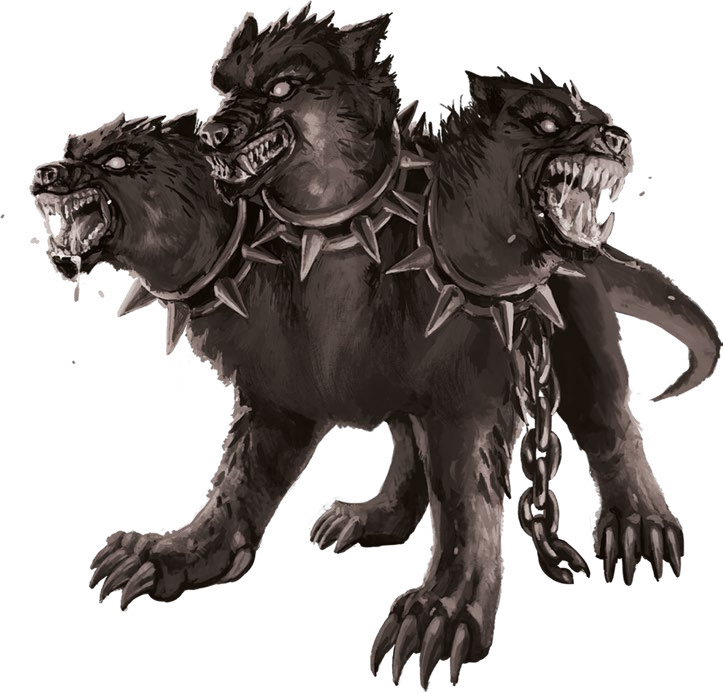
\includegraphics[width=0.85\paperwidth, keepaspectratio]{\art/cerberi.png}
  };
  \node(map)[anchor=center] at (current page.center) {
    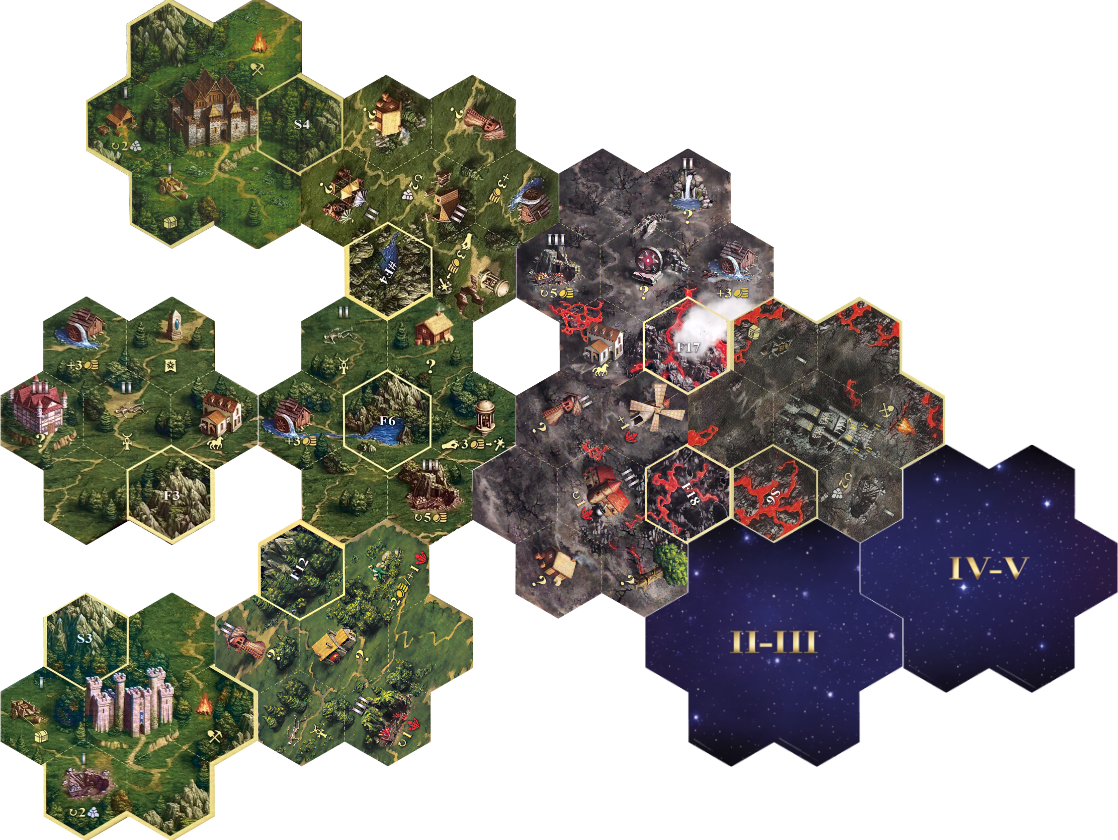
\includegraphics[width=\textwidth]{\_assets/maps/inferno_deal_with_the_devil.png}
  };

  
  \node at (1.5, -6) {\large{{\textbf{\textcolor{darkcandyapplered}{S4}}}}};
  \node at (7, -6) {\large{{\textbf{\textcolor{darkcandyapplered}{\#F4}}}}};
  \node at (12.6, -8.4) {\large{{\textbf{\textcolor{darkcandyapplered}{F17}}}}};
  \node at (15, -9.5) {\large{{\textbf{\textcolor{darkcandyapplered}{Kleesive}}}}};
  \node at (15, -10.3) {\large{{\textbf{\textcolor{darkcandyapplered}{S6}}}}};
  \node at (15.9, -16.8) {\large{{\textbf{\textcolor{darkcandyapplered}{N12}}}}};
  \node at (12.4, -18) {\large{{\textbf{\textcolor{darkcandyapplered}{F16}}}}};
  \node at (9.3, -15.6) {\large{{\textbf{\textcolor{darkcandyapplered}{F18}}}}};
  \node at (6, -18) {\large{{\textbf{\textcolor{darkcandyapplered}{F12}}}}};
  \node at (2, -19) {\large{{\textbf{\textcolor{darkcandyapplered}{S3}}}}};
  \node at (0.1, -13.3) {\large{{\textbf{\textcolor{darkcandyapplered}{F3}}}}};
  \node at (4.3, -10.3) {\large{{\textbf{\textcolor{darkcandyapplered}{F6}}}}};
\end{tikzpicture}
